\documentclass{beamer}

\usepackage{tikz}

\begin{document}

\begin{frame}

Images and diagrams for tensor spaces.

Creative Commons CC 4.0 by James B. Wilson (and others if they add their name).
\end{frame}

\begin{frame}
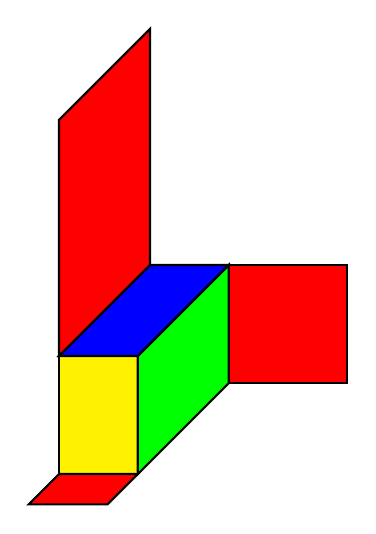
\begin{tikzpicture}[scale=0.25]
\pgfmathsetmacro{\cubex}{4}
\pgfmathsetmacro{\cubey}{6}
\pgfmathsetmacro{\cubez}{12}
\draw[black,thick,fill=yellow] (0,0,0) -- ++(-\cubex,0,0) -- ++(0,-\cubey,0) -- ++(\cubex,0,0) -- cycle;
\draw[black,thick,fill=green] (0,0,0) -- ++(0,0,-\cubez) -- ++(0,-\cubey,0) -- ++(0,0,\cubez) -- cycle;
\draw[black,thick,fill=blue] (0,0,0) -- ++(-\cubex,0,0) -- ++(0,0,-\cubez) -- ++(\cubex,0,0) -- cycle;
\draw[black, thick,fill=red] (0,-\cubey,0) -- ++(-\cubex,0,0) -- ++(0,0,\cubex) -- ++(\cubex,0,0) -- cycle;
\draw[black, thick,fill=red] (-\cubex,0,0) -- ++(0,0,-\cubez) -- ++(0,\cubez,0) -- ++(0,0,\cubez) -- cycle;
\draw[black, thick,fill=red] (0,0,-\cubez) -- ++(\cubey,0,0) -- ++(0,-\cubey,0) -- ++(-\cubey,0,0) -- cycle;
\end{tikzpicture}
\end{frame}


\begin{frame}
\begin{tikzpicture}[scale=0.75]
\pgfmathsetmacro{\xx}{2}
\pgfmathsetmacro{\yy}{2}
\pgfmathsetmacro{\zz}{-2}
\pgfmathsetmacro{\boxscale}{0.5}
\node (left) at (2.2,-0.5) {\begin{tikzpicture}[scale=\boxscale]
	% front
	\draw[black] (0,0,0)
			-- ++(\xx,0,0) -- ++(0,\yy,0) --++(-\xx,0,0) -- cycle;
	% side
	\draw[black] (\xx,0,0)
		-- ++(0,0,\zz) -- ++(0,\yy,0) --++(0,0,-\zz) -- cycle;
	% top
	\draw[black] (0,\yy,0) 
		-- ++(\xx,0,0) -- ++(0,0,\zz) --++(-\xx,0,0) -- cycle;	
		
	%Mat	
	\draw[black] (0,0,0) -- ++(0,0,-\zz) 
		--++(0,\yy,0) -- ++(0,0,\zz) -- cycle;
	\draw[black,fill=black!25] (0,0,0) -- ++(0,0,-\zz) 
		--++(0,\yy,0) -- cycle;
\end{tikzpicture}}; % (left)
\end{tikzpicture}
\end{frame}

\begin{frame}
\begin{tikzpicture}[scale=0.75]
\pgfmathsetmacro{\xx}{2}
\pgfmathsetmacro{\yy}{2}
\pgfmathsetmacro{\zz}{-2}
\pgfmathsetmacro{\boxscale}{0.5}


\node (d2) at (1.2,0.2) {$\delta_2$};
\node (t2) at (2.2,1.2) {$T$};
\node (left) at (2.2,-0.5) {\begin{tikzpicture}[scale=\boxscale]
	% front
	\draw[black] (0,0,0)
			-- ++(\xx,0,0) -- ++(0,\yy,0) --++(-\xx,0,0) -- cycle;
	% side
	\draw[black] (\xx,0,0)
		-- ++(0,0,\zz) -- ++(0,\yy,0) --++(0,0,-\zz) -- cycle;
	% top
	\draw[black] (0,\yy,0) 
		-- ++(\xx,0,0) -- ++(0,0,\zz) --++(-\xx,0,0) -- cycle;	
		
	%Mat	
	\draw[black] (0,0,0) -- ++(0,0,-\zz) 
		--++(0,\yy,0) -- ++(0,0,\zz) -- cycle;
	\draw[black,fill=black!25] (0,0,0) -- ++(0,0,-\zz) 
		--++(0,\yy,0) -- cycle;
\end{tikzpicture}}; % (left)

\node (minus) at (4.5,0) {$+$};

\node (d1) at (5.2,1.5) {$\delta_1^{\circ}$};
\node (t1) at (5.2,0.7) {$T$};
\node (mid) at (6,0.5) {\begin{tikzpicture}[scale=\boxscale]
	% front
	\draw[black] (0,0,0)
			-- ++(\xx,0,0) -- ++(0,\yy,0) --++(-\xx,0,0) -- cycle;
	% side
	\draw[black] (\xx,0,0)
		-- ++(0,0,\zz) -- ++(0,\yy,0) --++(0,0,-\zz) -- cycle;
	% top
	\draw[black] (0,\yy,0) 
		-- ++(\xx,0,0) -- ++(0,0,\zz) --++(-\xx,0,0) -- cycle;	

	% Mat
	\draw[black] (0,\yy,\zz) -- ++(\xx,0,0) 
		--++(0,\yy,0) -- ++(-\xx,0,0) -- cycle;
	\draw[black, fill=black!25] (0,\yy*2,\zz) -- ++(\xx,0,0) 
		--++(0,-\yy,0) -- cycle;
\end{tikzpicture}}; % (mid)

\node (minus) at (7.5,0) {$=$};

\node (d0) at (11,0) {$\delta_0$};
\node (t0) at (9.2,1.2) {$T$};
\node (mid) at (9.5,0) {\begin{tikzpicture}[scale=\boxscale]
	% front
	\draw[black] (0,0,0)
			-- ++(\xx,0,0) -- ++(0,\yy,0) --++(-\xx,0,0) -- cycle;
	% side
	\draw[black] (\xx,0,0)
		-- ++(0,0,\zz) -- ++(0,\yy,0) --++(0,0,-\zz) -- cycle;
	% top
	\draw[black] (0,\yy,0) 
		-- ++(\xx,0,0) -- ++(0,0,\zz) --++(-\xx,0,0) -- cycle;	

	% Mat
	\draw[black] (\xx,0,0) -- ++(\xx,0,0) 
		--++(0,0,\zz) -- ++(-\xx,0,0) -- cycle;
	\draw[black, fill=black!25] (\xx,0,0) -- ++(\xx,0,0) 
		--++(-\xx,0,\zz) -- cycle;
\end{tikzpicture}}; % (mid)

\node (imp) at (12,0) {$\Rightarrow$};
\node (answer) at (14,0) {\begin{tikzpicture}[scale=\boxscale]
	% front
	\draw[black, fill=black!25] (0,0,0)
		-- ++(\xx,0,\zz) -- ++(-\xx,\yy,0) -- cycle;
	% side
%	\draw[black, fill=black!25] (\xx,0,0)
%		-- ++(0,\yy,0) -- ++(0,-\yy,\zz) -- cycle;
	% top
	\draw[black,dotted] (0,0,0) -- ++(0,0,\zz) -- ++(0,\yy,0);
	\draw[black,dotted] (0,0,\zz) -- ++(\xx,0,0);

	% front
	\draw[black] (0,0,0)
			-- ++(\xx,0,0) -- ++(0,\yy,0) --++(-\xx,0,0) -- cycle;
	% side
	\draw[black] (\xx,0,0)
		-- ++(0,0,\zz) -- ++(0,\yy,0) --++(0,0,-\zz) -- cycle;
	% top
	\draw[black] (0,\yy,0) 
		-- ++(\xx,0,0) -- ++(0,0,\zz) --++(-\xx,0,0) -- cycle;	

\end{tikzpicture}}; % (answer)
\end{tikzpicture}
\end{frame}

\end{document}